% !TeX TXS-program:compile = txs:///pythonlualatex

\documentclass[a4paper,11pt]{article}
\usepackage[pythontex]{cp-base} %avec options possibles parmi breakable (tcbox), sujetl (exos),  (pour faire "comme avant"), etc...
\graphicspath{{./graphics/}}
%variables
\donnees[%
	typedoc=CHAPITRE~,
	numdoc=3,
	classe=1\up{ère} 2M2,
	matiere={[SPÉ.MATHS]},
	annee=2021,
	titre=Droites et fonctions affines
]

%formatage
\author{Pierquet}
\title{\nomfichier}
\hypersetup{pdfauthor={Pierquet},pdftitle={\nomfichier},allbordercolors=white,pdfborder=0 0 0,pdfstartview=FitH}
%divers
\lhead{\entete{\matiere}}
\chead{\entete{\lycee}}
\rhead{\entete{\classe{} - Chapitre \thepart}}
\lfoot{\pied{\matiere}}
\cfoot{\logolycee{}}
\rfoot{\pied{\numeropagetot}}

\begin{document}

\pagestyle{fancy}

\part{CH03 - Droites et fonctions affines}

\section{Généralités}

\subsection{Définition}

\begin{cdefi}
Une fonction $f$ est \textbf{affine} s'il existe deux réels $m$ et $p$ tels que $f(x)=mx+p$.

Son programme de calcul ne comporte qu'une multiplication (ou division) et une addition (ou soustraction).
\end{cdefi}

\begin{crmq}[s]
$\bullet~~$On utilise aussi souvent les notations $f(x)=ax+b$, qui sont parfois plus ambigües.

$\bullet~~$Si $m=0$, la fonction est \textbf{constante}.

$\bullet~~$Si $p=0$, la fonction est \textbf{linéaire} et traduit une situation de proportionnalité.
\end{crmq}

\subsection{Représentation graphique}

\begin{cprop}
La courbe représentative d'une fonction affine $f(x)=mx+p$ est toujours une \textbf{droite}.\\ L'équation réduite de cette droite est $y=mx+p$.

La constante \textbf{multiplicative} $m$ est la \textbf{pente} de la droite (appelée aussi \textbf{coefficient directeur}).

La constante \textbf{additive} $p$ s'appelle \textbf{ordonnée à l'origine} : c'est la valeur en laquelle la droite traverse l'axe des ordonnées.
\end{cprop}

\begin{crmq}
Inversement, une droite non verticale est toujours la représentation graphique d'une fonction affine.
\end{crmq}

\begin{cprop}
Si $A(x_A;y_A)$ et $B(x_B;y_B)$ sont deux points d'une droite, alors : \[m=\frac{y_B-y_A}{x_B-x_A}= \frac{\mbox{déplacement vertical}}{\mbox{déplacement horizontal}} \quad 	\mbox{(compter les déplacements en \emph{unités} et pas en carreaux)}\]
\end{cprop}

\begin{cmethode}
Pour \textbf{lire l'équation d'une droite}, il suffit de trouver $p$ et $m$ :
	\begin{itemize}
		\item On repère l'ordonnée à l'origine $p$, c'est-à-dire la valeur où la droite traverse l'axe des ordonnées
		\item On repère deux points de la droite assez éloignés et dont les coordonnées sont les plus précises possibles et on calcule $m$ avec la formule $m=\frac{\mbox{déplacement vertical}}{\mbox{déplacement horizontal}} = \frac{\Delta y}{\Delta x}$
\end{itemize}
\end{cmethode}

\begin{cexemple}
La droite tracée ci-dessous est la droite d'équation $y=3x-2$.

En effet :
\begin{itemize}[leftmargin=*]
	\item la droite traverse l'axe des ordonnées en $-2$ donc $p=-2$ ;
	\item quand on se décale de $\Delta x=1$ unité vers la droite, on se décale de $\Delta y=3$ unités vers le haut donc $m=\frac{3}{1}=3$.
\end{itemize} 
\end{cexemple}

\begin{cillustr}
\begin{center}
	\tunits{1}{0.6}
	\tdefgrille{-1}{5}{1}{1}{-3}{6}{1}{1}
	\begin{tikzpicture}[x=\xunit cm,y=\yunit cm]
		%axes et grille
		\tgrillep[line width=0.35pt,gray!50] ;
		\draw[->,line width=1.25pt] (\xmin,0) -- (\xmax,0);
		\draw[->,line width=1.25pt] (0,\ymin) -- (0,\ymax);
		\foreach \x in {-1,0,...,4}
			\draw[line width=1.25pt] (\x,4pt) -- (\x,-4pt) node[below] {\small \num{\x}};
		\foreach \y in {-3,-2,...,5}
			\draw[line width=1.25pt] (4pt,\y) -- (-4pt,\y) node[left] {\small \num{\y}};
		%fonction
		\clip (\xmin,\ymin) rectangle (\xmax,\ymax);
		\draw[line width=1.25pt,red,domain=\xmin:\xmax,samples=200] plot(\x,{3*\x-2});
		%données
		\foreach \Point in {(0,-2),(1,1),(2,4)}
			\draw[ultra thick,blue] plot[mark=+,mark size=4pt] coordinates {\Point};
		\draw (0,-2) node[right] {$p$ (ici $-2$)};
		\draw[line width=1pt,->] (1,1) -- (2,1) node[midway,below] {$\Delta x=1$} ;
		\draw[line width=1pt,->] (2,1) -- (2,4) node[midway,right] {$\Delta y=3$} ;
	\end{tikzpicture}
\end{center}

\begin{calgo}
En \calgpython, on peut créer une \calg{fonction} permettant de calculer les valeurs de $m$ et de $p$ :
	
	\begin{tcpythoncode}[15cm]
		\begin{pyverbatim}[][fontsize=\footnotesize,numbers=left,numbersep=10pt]
			from math import *
			def eqdroite(xA,yA,xB,yB) :
				if xA == xB :            #la droite est verticale !
					return None
				m = (yB-yA)/(xB-xA)
				p = yB - m*xB
				return m,p
		\end{pyverbatim}
	\end{tcpythoncode}
	
\begin{pyconcode}
from math import *
def eqdroite(xA,yA,xB,yB):
	m = (yB-yA)/(xB-xA)
	p = yB - m*xB
	return m,p
	

\end{pyconcode}
	
\begin{consolepython}[15cm]
\begin{pyconsole}[][framesep=3mm,frame=single,label={[\scriptsize Début de la console \logopython]\scriptsize Fin de la console \logopython},fontsize=\footnotesize,framerule=1pt,rulecolor=\color{ForestGreen}]
eqdroite(1,1,2,4) #droite passant par (1,1) et (2,4)
\end{pyconsole}
\end{consolepython}
\end{calgo}
%
%
%	\begin{minipage}[t]{0.65\linewidth}
%		\vspace{0pt}
%		
%		\vspace{0.5cm}\underline{Exercice} : Trouver l'équation de la droite passant par les points $A(2;5)$ et $B(7;-1)$.
%		
%	\end{minipage} \hfill
%	\begin{minipage}[t]{0.32\linewidth}
%		\vspace{0pt}
%		\psset{showpoints=false, % affichage des points
%			dotstyle=+, % style de point
%			dotsize=6pt, % taille de point
%			linewidth=0.8pt, % ´epaisseur des traits
%			subgriddiv=1, % grille divis´ee aux unit´es
%			griddots=100, % nombre de points sur le cˆot´e du carreau
%			gridlabels=0, % taille des ´etiquettes
%			gridwidth=0.8pt, % ´epaisseur du trait de quadrillage
%			xunit=1, % facteur d’unit´e en abscisse
%			yunit=1, % facteur d’unit´e en ordonn´ee
%			runit=0.5, % facteur d’unit´e en radial
%			gridcolor=lightgray, % couleur de la grille
%			arrowsize=3pt 2, % taille de la flèche ?
%			arrowinset=0.25} % taille de la pointe de la flèche
%		
%		\begin{pspicture}(-1,-3)(5,6)
%			\psgrid \psaxes[labelFontSize=\scriptstyle,xAxis=true,yAxis=true,Dx=1,Dy=1,ticksize=-2pt]{->}(0,0)(-1,-3)(5,6)	
%			\psline[showpoints=false](-0.333,-3)(2.667,6)
%			\psline{->}(1,1)(2,1)
%			\psline{->}(2,1)(2,4)
%			\psdot(0,-2)
%			\uput[r](0,-2){$p$ (ici -2)}
%			\psdot(1,1)
%			\psdot(2,4)
%			\uput[d](1.5,1){\small $\Delta x=1$}
%			\uput[r](2,2.5){$\Delta y=m$ (ici 3)}
%		\end{pspicture}
%	\end{minipage}%
\end{cillustr}

\begin{crmq}
On peut également travailler de manière algébrique pour déterminer $p$ (si on connaît $m$) grâce à :
\begin{itemize}
	\item $p=y_A-m \times x_A$ ;
	\item $p=y_B-m \times x_B$ ;
\end{itemize}
\end{crmq}

\subsection{Tracé}

\begin{cmethode}[ 1]
Pour \textbf{tracer} la droite représentative d'une fonction affine (ou une droite d'équation donnée):
	\begin{itemize}
		\item On choisit deux valeurs $x_A$ et $x_B$ assez éloignées
		\item On calcule les images $y_A=mx_A+p$ et $y_B=mx_B+p$ 
		\item On place les points $A$ et $B$ correspondants et on trace à la règle la droite $(AB)$.
\end{itemize}
\end{cmethode}

\begin{cmethode}[ 2]
Pour \textbf{tracer} la droite représentative d'une fonction affine (ou une droite d'équation donnée):
	\begin{itemize}
		\item On place le point d'ordonnée $p$ sur l'axe des ordonnées.
		\item Depuis ce point, on se décale de 1 unité en abscisse, puis de $m$ unités en ordonnées : on obtient un deuxième point de la droite (et éventuellement on recommence).
		\item On relie ces points à la règle.
\end{itemize}
\end{cmethode}

\newpage

\section{Sens de variations, signe d'une fonction affine}

\subsection{Sens de variation}

\begin{cprop}
Une fonction affine est toujours \textbf{monotone}, et son sens de variation est donné par le \textbf{signe} de son coefficient directeur $m$ :
	\begin{itemize}
		\item Si $m$ est \textbf{positif}, la fonction est \textbf{croissante}.
		\item Si $m$ est \textbf{négatif}, la fonction est \textbf{décroissante}.
\end{itemize}
\end{cprop}

\begin{calgo}
En \calgpython, on peut créer une \calg{fonction} permettant de retourner le sens de variation d'une fonction affine :

\begin{tcpythoncode}[15cm]
	\begin{pyverbatim}[][fontsize=\footnotesize,numbers=left,numbersep=10pt]
		from math import *
		def variation(m,p):
			if m == 0 :
				var = "constante"
			elif m>0 :
				var = "croissante"
			else :
				var = "décroissante"
			return var
	\end{pyverbatim}
\end{tcpythoncode}

\begin{pyconcode}
from math import *
def variation(m,p):
	if m == 0 :
		var = "constante"
	elif m>0 :
		var = "croissante"
	else :
		var = "décroissante"
	return var
	
	
\end{pyconcode}

\begin{consolepython}[15cm]
\begin{pyconsole}[][framesep=3mm,frame=single,label={[\scriptsize Début de la console \logopython]\scriptsize Fin de la console \logopython},fontsize=\footnotesize,framerule=1pt,rulecolor=\color{ForestGreen}]
variation(2,3), variation(-2,-1), variation(0,3)
\end{pyconsole}
\end{consolepython}
\end{calgo}

\subsection{Signe}

\begin{cprop}
Si une fonction affine $f$ n'est pas constante, sa droite représentative n'est pas horizontale donc elle traverse toujours une seule fois l'axe des abscisses. On trouve cette racine en résolvant l'équation $f(x)=0$.
\end{cprop}

\begin{cmethode}
Pour dresser le tableau de signes d'une fonction affine :
	\begin{itemize}[leftmargin=*]
		\item On cherche sa racine en résolvant $f(x)=0$.
		\item  Pour trouver le signe de $f(x)$ de part et d'autre de cette racine, on regarde  le signe de $m$, qui donne les variations de $f$ : si elle est croissante, elle ira du $\ominus$ vers le $\oplus$ et si elle est décroissante, elle ira du $\oplus$ vers le $\ominus$.
	\end{itemize}
\end{cmethode}

\begin{cexemple}
La fonction $f$ définie par $f(x)=3x-2$ tracée ci-dessus a pour tableau de signes :
\begin{center}
	\begin{tikzpicture}
		\tkzTabInit{$x$ / 1.1, $3x-2$ / 1.4}{$-\infty$, $\frac{2}{3}$, $+\infty$}
		\tkzTabLine{, -, z, +, }
	\end{tikzpicture}
\end{center}
En effet, elle s'annule lorsque $3x-2=0$ c'est-à-dire lorsque $x=\nicefrac{2}{3}$.\\ La pente de la droite est $m=3$ qui est positif, donc elle est croissante et va du $\ominus$ vers le $\oplus$.
\end{cexemple}

\begin{crmq}[s]
Si une fonction affine est constante, elle est toujours du même signe, celui de $p$ !

\smallskip

Le fait de savoir déterminer le tableau de signes d'une fonction \og du premier degré \fg{} permet, grâce à un tableau de signes, de pouvoir déterminer le signe d'une fonction se présentant sous la forme :

\hfill~d'un ensemble de produit(s)/quotient(s) de facteurs du 1\up{er} degré.\hfill~
\end{crmq}

\begin{calgo}
En \calgpython, on peut créer une \calg{préocédure} permettant d'afficher le signe de $mx+p$ :

\begin{tcpythoncode}[15cm]
	\begin{pyverbatim}[][fontsize=\footnotesize,numbers=left,numbersep=10pt]
		from math import *
		def signe(m,p) :
			if m==0 :
				if p>=0 :
					signe = '+'
				else :
					signe = '-'
				print(f"mx+p est du signe de p, soit ici {signe}")
			elif m>0 :
				racine , signe = -p/m , '-0+'
				print(f"mx+p s'annule en {racine} et son signe est {signe}")
			else :
				racine , signe = -p/m , '+0-'
				print(f"mx+p s'annule en {racine} et son signe est {signe}")
	\end{pyverbatim}
\end{tcpythoncode}

\begin{pyconcode}
def signe(m,p):
	if m==0 :
		if p>=0 :
			signe = '+'
		else :
			signe = '-'
		print(f"mx+p est du signe de p, soit ici {signe}")
	elif m>0 :
		racine = -p/m
		signe = '-0+'
		print(f"mx+p s'annule en {racine} et son signe est {signe}")
	else :
		racine = -p/m
		signe = '+0-'
		print(f"mx+p s'annule en {racine} et son signe est {signe}")
	
	
\end{pyconcode}

\begin{consolepython}[15cm]
\begin{pyconsole}[][framesep=3mm,frame=single,label={[\scriptsize Début de la console \logopython]\scriptsize Fin de la console \logopython},fontsize=\footnotesize,framerule=1pt,rulecolor=\color{ForestGreen}]
signe(2,3)
signe(-2,-1)
signe(0,5)
\end{pyconsole}
\end{consolepython}
\end{calgo}

\section{Compléments - Tableaux de signes, inéquations}

\begin{crappel}[s]
Pour créer le \textbf{tableau de signes} d'une expression, il faut très souvent penser à respecter une règle essentielle (\textit{règle des signes}) : l'expression doit se présenter sous forme de produit(s)/quotient(s).

\smallskip

Si ce n'est pas le cas, on peut essayer de \textit{transformer} pour se ramener à la configuration produit(s)/quotient(s). Pour cela il existe deux \textbf{techniques} de base : \textbf{factoriser} et/ou \textbf{mettre au même dénominateur}.
\end{crappel}

\begin{crappel}[s]
Pour résoudre une inéquation, on peut travailler en utilisant un tableau de signes. Toutefois, avant de se lancer directement dans la création du tableau, il faut s'assurer qu'on cherche à résoudre \og plus grand ou plus petit que \textbf{0} ! \fg{}

\smallskip

Si ce n'est pas le cas, on commence déjà par se ramener à : \og $\pg 0$ \fg, \og $\pp 0$ \fg, \og $> 0$ \fg ou \og $< 0$ \fg.

\smallskip

On peut ensuite de reporter au point précédent, et se ramener (si besoin) à une forme produit(s)/quotient(s).

\medskip

\hfill\textsf{On peut retenir cette méthode grâce à l'acronyme \textbf{ZPQ} : \textbf{Z}éro \& \textbf{P}roduit \& \textbf{Q}uotient.}\hfill~
\end{crappel}

\end{document}